\newpage
\hypertarget{stringRep tex}{}
\subsection{Implementing toString for \texttt{Box}}
\texHeader

\vspace{0.5cm}

\begin{itemize}
  
\item[$\blacktriangleright$] Closely following Fig.~\ref{fig:goal_stringRep}, create a nested \texttt{forEach} loop in \texttt{Box.toString()}.
Don't worry about invoking \texttt{addToStringRep} yet -- just make sure you return the \texttt{this.stringRep} attribute. It should resemble
Fig.~\ref{fig:emptyLoops}. \texttt{this.stringRep} is referred to as an \emph{AttributeValueExpression}\defineMOSL{AttributeValueExpression} as it accesses an
attribute value of an object variable (\texttt{this}) via a `.' (dot) operator.

\begin{figure}[htp]
\begin{center}
  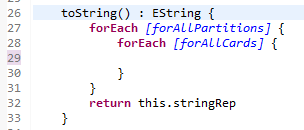
\includegraphics[width=0.5\textwidth]{eclipse_toStringNestedLoops}
  \caption{Control flow for \texttt{toString} with nested \emph{for each} loops}
  \label{fig:emptyLoops}
\end{center}
\end{figure}

\item[$\blacktriangleright$] In order to invoke \texttt{addToStringRep}, we need a \emph{statement node}. Remembering that statement nodes are enclosed in
\texttt{< >}, write inside the second loop: \syntax{<@this.addToStringRepCard(card)>} 
The correct \texttt{card} parameter will be matched by the \texttt{forAllCards} pattern. We'll establish this in a moment.

\vspace{0.5cm}

\item[$\blacktriangleright$] The completed \texttt{toString} activity should now resemble Fig.~\ref{fig:toStringFlow}.

\vspace{0.5cm}

\begin{figure}[htp]
\begin{center}
  \includegraphics[width=0.6\textwidth]{eclipse_boxtoStringFlow}
  \caption{Using a \emph{statement node} to invoke a void helper method}
  \label{fig:toStringFlow}
\end{center}
\end{figure}

\item[$\blacktriangleright$] Don't forget that the aim of the activity is to access every card in \texttt{Box}. The control flow terminates when the helper
method has been called for all existing cards. This means the \texttt{forAllPartitions} and \texttt{forAllCards} patterns must match all cards in all
partitions.

\clearpage

\item[$\blacktriangleright$] Complete each pattern as depicted in Fig.~\ref{fig:toStringPatterns}. The \texttt{partition} in \texttt{forAllCards} is bound to
the one matched in the current (first) loop iteration, but \texttt{card} is \emph{not} bound as it must be newly matched each time.

\vspace{0.5cm}

\begin{figure}[htp]
\begin{center}
  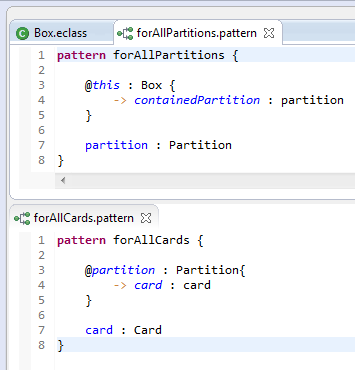
\includegraphics[width=0.6\textwidth]{eclipse_toStringPatterns}
  \caption{Box traversal patterns}
  \label{fig:toStringPatterns}
\end{center}
\end{figure}

\vspace{0.5cm}

\item[$\blacktriangleright$] As crazy at it may seem, that's it!  To see how this SDM is represented visually, check out Fig.~\ref{fig:sdm_tostring_5}.

\end{itemize}
